\chapter{Outillage du développeur}
\label{chap-dev-tooling}

\renewcommand{\headrulewidth}{0.3pt}
\fancyhead[LE]{\thepage} \fancyhead[RE]{\nouppercase{\textbf{\leftmark}}}
\fancyhead[RO]{\thepage} \fancyhead[LO]{\nouppercase{\textbf{\rightmark}}}
\fancyfoot[L,C,R]{}

\setlength{\parindent}{0.35cm}

\minitoc
\newpage
% ================================================================

Ce chapitre couvre les \textbf{outils optionnels} qui facilitent le développement au quotidien : les utilitaires de débogage (rechargement du plug-in, inspection des erreurs, et un débogueur VS-Code complet attaché à QGIS), et \script{Qt Designer} pour la création des boîtes de dialogue.

\section{Outils de débogage}
\subsection{L'extension \script{Plugin Reloader}}

Cet utilitaire permet de recharger une extension après une modification de code. Il n'est ainsi pas nécessaire de relancer QGIS après chaque changement de code.

L'extension peut être installée depuis le gestionnaire d'extensions de \script{QGIS}.

\begin{figure}[H]
    \centering
    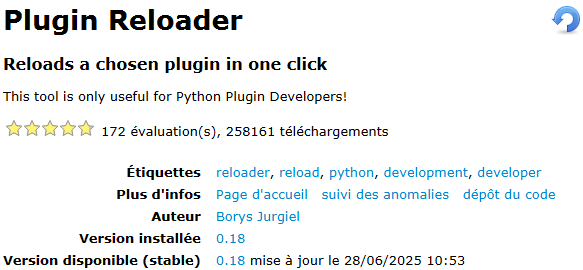
\includegraphics[width=0.75\linewidth]{9_developer_tooling/fig/plugin_reloader.png}
    \caption{Fiche descriptive de \script{Plugin Reloader}}
    \label{fig_plugin_reloader}
\end{figure}

\subsection{L'extension QGIS \script{First Aid}}

L'extension \script{First Aid} permet d'investiguer les erreurs survenant lors de l'exécution de l'extension.


\newpage
\subsection{VS-Code}
L'extension \script{debugvs} permet de connecter une instance de débogage \script{VS-Code} à l'exécution de l'extension depuis QGIS. Cette configuration de débogage permet d'utiliser toutes les fonctionnalités de VS Code pendant le débogage (points d'arrêt, watch, pile d'appels...). La mise en place de cette configuration de débogage se fait comme suit :
\begin{enumerate}
    \item installez \script{debugpy} avec la commande \script{!pip install debugpy} depuis l'invite de commande Python de QGIS ;
    \item \sloppy si le répertoire de développement de l'extension n'est pas situé dans \texttt{C://Users/$USER$/AppData//QGIS/QGIS3/profiles/default/python}, créez un lien symbolique dans ce répertoire pointant vers le répertoire de développement.
    \item installez l'extension \script{debugvs} en téléchargeant son script depuis le dépôt GitLab \url{https://github.com/lmotta/debug_vs} et activez l'extension en important le dossier \script{.zip} dans \script{QGIS} (\cffig \ref{fig_debugvs}) ;
    \begin{figure}[H]
        \centering
        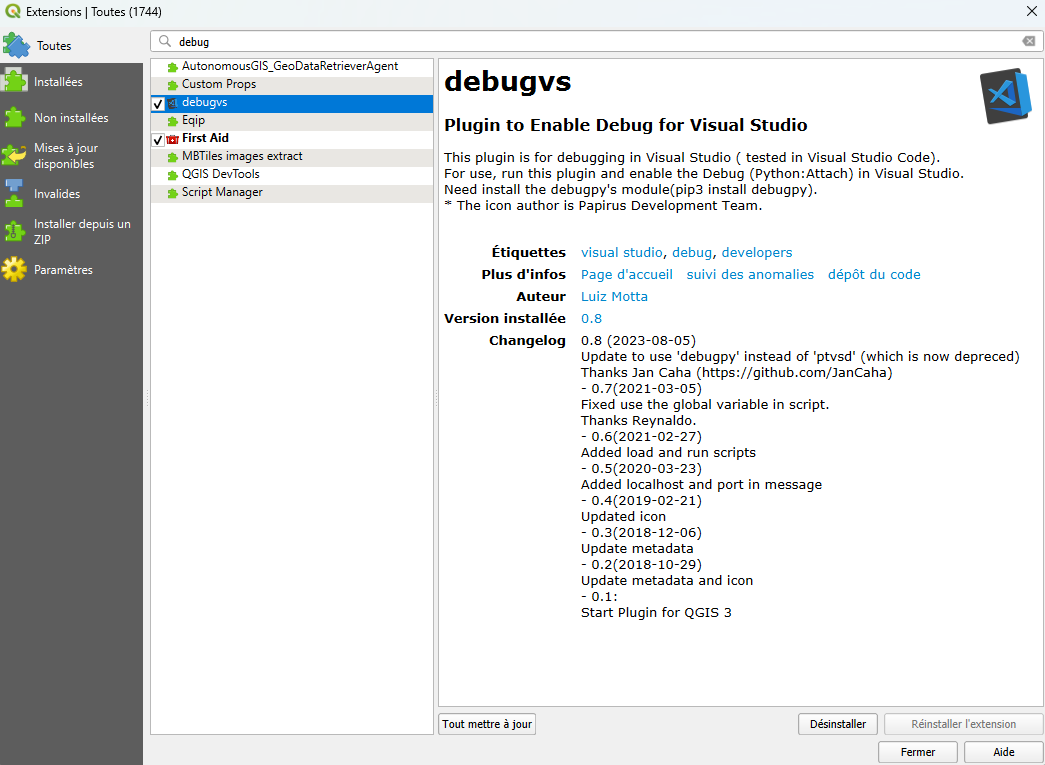
\includegraphics[width=0.6\linewidth]{9_developer_tooling/fig/debugvs.png}
        \caption{Extension \script{debugvs}}
        \label{fig_debugvs}
    \end{figure}
    \item configurez VS Code pour se connecter à QGIS pendant une session de débogage :
    \begin{enumerate}
        \item dans le répertoire de développement CaWaQS-Viz, créez un sous-répertoire \script{.vscode} (ajoutez ce répertoire au fichier \script{.gitignore}) ;
        \item créez un fichier \script{settings.json} dans le sous-répertoire \script{.vscode} et copiez le contenu du code \ref{code_settings_vscode}. Modifiez éventuellement les chemins des répertoires pour correspondre à votre installation QGIS et Python et à votre système d'exploitation. Celui-ci est pour Windows.
        \begin{lstlisting}[language=JSON, caption={Fichier de configuration du workspace. Ce fichier définit la configuration du workspace Visual Studio Code pour le développement d'extensions QGIS. Il adapte l'environnement Python de VS Code à celui utilisé par QGIS (installé via OSGeo4W).}, label=code_settings_vscode]
        {

            "workbench.colorCustomizations": {
                "titleBar.activeBackground": "#006823",
                "editor.background": "#000000"
            },

            "python.linting.pylintEnabled": true,
            "python.jediEnabled": true,


            "python.pythonPath": "C:/OSGeo4W64/bin/python-qgis.bat",


            "python.linting.pylintArgs": [
                "--extension-pkg-whitelist=PyQt5,qgis,db_manager",
                "--disable=all",
                "--enable=F,E,unreachable,duplicate-key,unnecessary-semicolon,global-variable-not-assigned,unused-variable,binary-op-exception,bad-format-string,anomalous-backslash-in-string,bad-open-mode"
            ],


            "terminal.integrated.env.windows": {

                "PATH": "C:\\OSGeo4W\\apps\\qgis\\bin;C:\\OSGeo4W\\apps\\Python312;C:\\OSGeo4W\\apps\\Python312\\Scripts;C:\\OSGeo4W\\apps\\Qt5\\bin;C:\\OSGeo4W\\apps\\Python312\\Scripts;C:\\OSGeo4W\\bin;C:\\Windows\\System32;C:\\Windows;C:\\Windows\\system32\\WBem;C:\\OSGeo4W\\apps\\Python312\\lib\\site-packages\\pywin32_system32;C:\\OSGeo4W\\apps\\Python312\\lib\\site-packages\\numpy\\.libs",

                "PYTHONHOME": "C:\\OSGeo4W\\apps\\Python312",
                "PYTHONPATH": "C:\\OSGeo4W\\apps\\qgis\\python;%PYTHONPATH%",

                "GDAL_DATA": "C:\\OSGeo4W\\share\\gdal",
                "GDAL_DRIVER_PATH": "C:\\OSGeo4W\\bin\\gdalplugins",
                "GDAL_FILENAME_IS_UTF8": "YES",

                "GEOTIFF_CSV": "C:\\OSGeo4W\\share\\epsg_csv",

                "O4W_QT_BINARIES": "C:/OSGeo4W/apps/Qt5/bin",
                "O4W_QT_DOC": "C:/OSGeo4W/apps/Qt5/doc",
                "O4W_QT_HEADERS": "C:/OSGeo4W/apps/Qt5/include",
                "O4W_QT_LIBRARIES": "C:/OSGeo4W/apps/Qt5/lib",
                "O4W_QT_PLUGINS": "C:/OSGeo4W/apps/Qt5/plugins",
                "O4W_QT_PREFIX": "C:/OSGeo4W/apps/Qt5",
                "O4W_QT_TRANSLATIONS": "C:/OSGeo4W/apps/Qt5/translations",
                "QT_PLUGIN_PATH": "C:\\OSGeo4W\\apps\\qgis\\qtplugins;C:\\OSGeo4W\\apps\\Qt5\\plugins",

                "QGIS_PREFIX_PATH": "C:/OSGeo4W/apps/qgis",

                "VSI_CACHE": "TRUE",
                "VSI_CACHE_SIZE": "1000000"
            },
            "python.languageServer": "Jedi",
        }
\end{lstlisting}
        \item créez un fichier \script{launch.json} dans le sous-répertoire \script{.vscode}, copiez le contenu du code \ref{code_launch_vscode}, modifiez les chemins \script{localRoot} et \script{remoteRoot} pour correspondre à la configuration de votre workspace.

        \begin{lstlisting}[language=JSON, caption={Fichier de configuration du débogueur VS-Code. Dans cette configuration, la section « connect » indique l'adresse et le port sur lesquels QGIS expose la session de débogage (ici localhost:5678). Le bloc « pathMappings » établit la correspondance entre les chemins locaux du projet ouverts dans VS Code (localRoot) et les chemins utilisés par QGIS pour exécuter l'extension (remoteRoot). Cette correspondance est essentielle pour que les points d'arrêt placés dans VS Code soient correctement associés aux fichiers réellement exécutés par QGIS.}, label = code_launch_vscode]
{
    "version": "0.2.0",
    "configurations": [
        {
            "name": "Attach QGIS Debug",
            "type": "python",
            "request": "attach",
            "connect": {
                "host": "localhost",
                "port": 5678
            },
            "pathMappings": [
                {
                    "localRoot": "C:\\Program Files\\$QGIS$\\apps\\qgis-ltr\\python\\plugins\\cawaqsviz",
                    "remoteRoot": "C:\\Users\\$USER$\\AppData\\Roaming\\QGIS\\QGIS3\\profiles\\default\\python\\cawaqsviz"
                }
            ],
            "justMyCode": false
        }
    ]
}


\end{lstlisting}
        \end{enumerate}
    \item Établissez la connexion QGIS/VS-Code
    \begin{enumerate}
        \item autorisez la connexion du débogueur à QGIS via l'extension \script{debugvs} (\cffig \ref{fig_enable_vscode_qgis}) ;
        \begin{figure}[H]
            \centering
            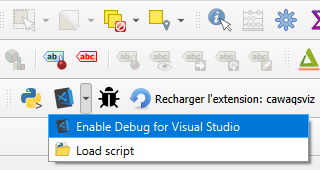
\includegraphics[width=0.40\linewidth]{9_developer_tooling/fig/launch_debug_vs.png}
            \caption{Établissement d'une connexion QGIS/VS-Code depuis l'extension \script{debugvs}}
            \label{fig_enable_vscode_qgis}
        \end{figure}
        \item lancez la session de débogage VS-Code (\cffig \ref{fig_debug_VS_CODE}).
        \begin{figure}[H]
            \centering
            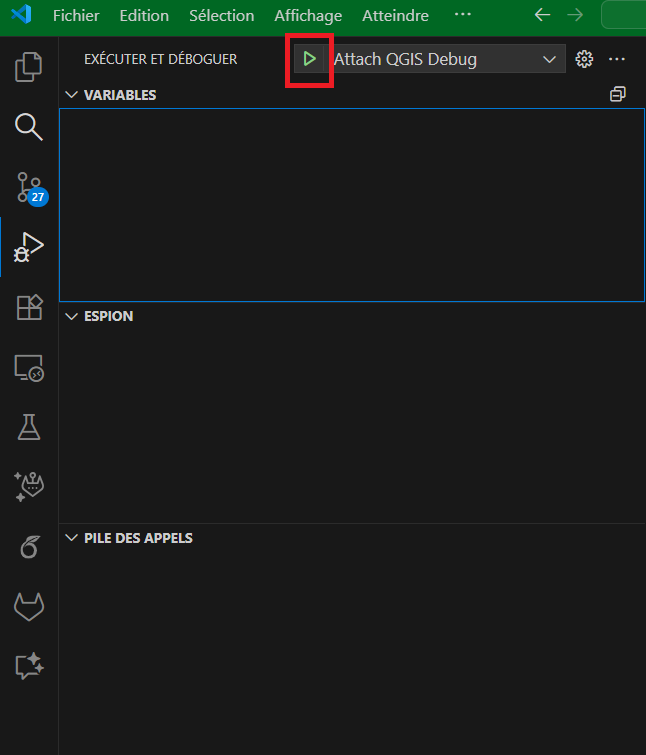
\includegraphics[width=0.5\linewidth]{9_developer_tooling/fig/debug_vs_code.png}
            \caption{Lancement d'une session de débogage depuis VS-Code}
            \label{fig_debug_VS_CODE}
        \end{figure}
    \end{enumerate}
\end{enumerate}

La connexion entre le débogueur et QGIS est terminée depuis VS-Code en cliquant sur \script{"Disconnected"} dans la barre d'outils de débogage (\cffig \ref{fig_barre_outil_debbug})

\begin{figure}[H]
    \centering
    
\includegraphics[width=0.35\linewidth]{9_developer_tooling/fig/disconnect-debugger.png}
    \caption{Barre d'outils du débogueur VS-Code}
    \label{fig_barre_outil_debbug}
\end{figure}




\newpage
\section{Créer des boîtes de dialogue avec \script{Qt Designer}}
\label{sec_QtDesigner}
L'application \script{Qt Designer}, fournie avec l'installation de QGIS (installation avec OSGEO), est un outil de création de boîtes de dialogue sous forme de fichiers .ui. Dans l'application \cwv, toutes les boîtes de dialogue disposent de leur propre fichier \script{.py} auquel le fichier \script{.ui}, de même nom, est associé à la classe Python de la boîte de dialogue.

\begin{lstlisting}[language = Python, label = code_init_from_ui, caption = Initialisation de la boîte de dialogue "Compare SIM/OBS" depuis un fichier .ui]
# This loads your .ui file so that PyQt can populate your plugin with the elements from Qt Designer
FORM_CLASS, _ = uic.loadUiType(
    os.path.join(os.path.dirname(__file__), "DialogComparesimobs.ui")
)


class DialogComparesimobs(Dialog, FORM_CLASS):
    def __init__(self, iface:QgisInterface, log_file_path:str, parent=None):
        """Constructor Method

        :param iface: Qgis Interface
        :type iface: QgisInterface
        :param logFilePath: Path of the cawaqs-viz log file, defaults to None
        :type logFilePath: str, optional
        :param parent: Parent class, defaults to None
        :type parent: _type_, optional
        """
        super(DialogComparesimobs, self).__init__(parent)
        self.setupUi(self)
        self.iface = iface
        self.logFilePath = log_file_path
        self.simData = False
\end{lstlisting}
